
\section{Architecture Integration}

\subsection{Model Support Matrix}

\begin{table}[H]
\centering
\small
\begin{tabular}{llllll}
\toprule
\textbf{Architecture} & \textbf{Attention} & \textbf{Nested?} & \textbf{RoPE?} & \textbf{GQA?} & \textbf{Path} \\
\midrule
DistilBERT & \texttt{MultiHeadSelfAttention} & No & No & No & Bidirectional \\
RoBERTa & \texttt{BertSelfAttention} & Yes & No & No & Bidirectional \\
GPT-2 & \texttt{GPT2Attention} & No & No & No & Causal \\
Qwen3.5 & \texttt{Qwen3Attention} & No & Yes & Yes & Causal \\
\bottomrule
\end{tabular}
\end{table}

\subsection{Weight Transfer}

\subsubsection{GPT-2 (Fused Conv1D)}

\begin{lstlisting}
if hasattr(old\_attn, "c\_attn"):
    c\_w = old\_attn.c\_attn.weight.data
    if "Conv1D" in cls\_c or hasattr(old\_attn.c\_attn, "nf"):
        c\_w = c\_w.t()
    split\_size = c\_w.size(0) // 3
    extracted["q"] = c\_w[:split\_size, :]
    extracted["k"] = c\_w[split\_size:2*split\_size, :]
    extracted["v"] = c\_w[2*split\_size:, :]
\end{lstlisting}

\subsubsection{RoBERTa (Nested)}

\begin{lstlisting}
elif hasattr(old\_attn, "self") and hasattr(old\_attn.self, "query"):
    extracted["q"] = old\_attn.self.query.weight.data
    extracted["k"] = old\_attn.self.key.weight.data
    extracted["v"] = old\_attn.self.value.weight.data
    extracted["o"] = old\_attn.output.dense.weight.data
\end{lstlisting}

\subsubsection{DistilBERT (Flat)}

\begin{lstlisting}
else:
    extracted["q"] = old\_attn.q\_lin.weight.data
    extracted["k"] = old\_attn.k\_lin.weight.data
    extracted["v"] = old\_attn.v\_lin.weight.data
    extracted["o"] = old\_attn.out\_lin.weight.data
\end{lstlisting}

\subsubsection{The Z Projection}

The \textbf{Z projection} is new. We initialize from $W_Q$:

\begin{lstlisting}
self.z\_proj.weight.data[:out\_z, :in\_z].copy\_(w\_q[:out\_z, :in\_z])
\end{lstlisting}

\subsection{Nested Encoder Detection}

The detection order:

\begin{lstlisting}
if (hasattr(old\_attn, "self") and hasattr(old\_attn.self, "query")
    and hasattr(old\_attn, "output") and hasattr(old\_attn.output, "dense")):
    is\_nested = True
elif cls\_name in ("BertSelfAttention", "RobertaSelfAttention", ...):
    is\_nested = True
elif model\_type in ("roberta", "bert", "xlm-roberta") and not is\_decoder:
    is\_nested = True
\end{lstlisting}

For nested encoders, \texttt{forward} returns raw context without \texttt{out\_proj}.

\subsection{GQA Support}

\begin{lstlisting}
if self.num\_kv\_heads != self.num\_heads:
    k = repeat\_kv(k, self.kv\_repeat)
    v = repeat\_kv(v, self.kv\_repeat)
\end{lstlisting}

\subsection{RoPE Support}

Handled via partial-dimension slicing:

\begin{lstlisting}
rotary\_dim = cos.shape[-1]
if rotary\_dim \textless{} head\_dim:
    q\_rot, q\_pass = q[..., :rotary\_dim], q[..., rotary\_dim:]
    q\_rot\_embed = q\_rot * cos + rotate\_half(q\_rot) * sin
    q = torch.cat([q\_rot\_embed, q\_pass], dim=-1)
\end{lstlisting}

\subsection{Injection Algorithm}

\textbf{Algorithm 2:} Inject Gated DeltaNet into a model
\begin{lstlisting}
Input:  model M, config c
Output: M with all attention replaced

1: layer\_list $\leftarrow$ find\_transformer\_layers(M)
2: for   in layer\_list:
3:     src $\leftarrow$ extract\_attention( )
4:     new $\leftarrow$ GatedDeltaNet(c, old=src)
5:     new.copy\_weights(src)
6:     replace\_attention( , new)
7: return M
\end{lstlisting}

\subsection{The Chunked Recurrence}

The core implementation is \texttt{chunked\_delta\_rule\_scan}:

\begin{lstlisting}
def chunked\_delta\_rule\_scan(q, k, v, beta, alpha, chunk\_size=8):
    # Normalize
    k\_unit = k / k.norm(dim=-1, keepdim=True).clamp(min=1e-6)
    q\_unit = q / q.norm(dim=-1, keepdim=True).clamp(min=1e-6)
    
    # Reshape into chunks
    q\_c = q\_unit.view(B, H, num\_chunks, chunk\_size, d)
    ...
    
    S = torch.zeros(B, H, d, d)  # state
    outputs = []
    
    for c in range(num\_chunks):       # $\leftarrow$ OUTER PYTHON LOOP
        q\_i, k\_i, v\_i = q\_c[:,:,c], k\_c[:,:,c], v\_c[:,:,c]
        if use\_checkpoint:
            y\_i, S = checkpoint(\_delta\_chunk\_forward, S, q\_i, k\_i, v\_i, ...)
        else:
            y\_i, S = \_delta\_chunk\_forward(S, q\_i, k\_i, v\_i, ...)
        outputs.append(y\_i)
    
    return torch.cat(outputs, dim=2)

def \_delta\_chunk\_forward(S, q\_i, k\_i, v\_i, beta\_i, alpha\_i):
    for t in range(chunk\_size):       # $\leftarrow$ INNER PYTHON LOOP
        kt, vt, qt = k\_i[:,:,t:t+1], v\_i[:,:,t:t+1], q\_i[:,:,t:t+1]
        bt, at = beta\_i[:,:,t:t+1], alpha\_i[:,:,t:t+1]
        
        inter\_v = torch.matmul(kt, S)
        err = vt - inter\_v
        norm\_k\_sq = (kt * kt).sum(-1, keepdim=True)
        step = (at / (1 + norm\_k\_sq).clamp(min=1.0)).clamp(0, 1)
        
        S = bt * S + step * torch.matmul(kt.transpose(-1, -2), err)
        yt = torch.matmul(qt, S)
    
    return torch.cat(outputs, dim=2), S
\end{lstlisting}

\textbf{Total Python iterations per forward:}
\[
L/C \text{ (outer)} + L/C \times C \text{ (inner)} = 2L/C + L \approx 2L
\]

For $L = 128$: \textbf{256 Python-level iterations per head per layer per forward}.

\subsection{Common Pitfalls}

\subsubsection{Python Loop Overhead}

Each \texttt{for} iteration involves:
\begin{itemize}
\item Tensor slicing (allocates new tensor)
\item Kernel launch (~5-10  s)
\item Python dispatch (~1-2  s)

\end{itemize}
For 256 iterations $\times$ 5 ops = ~1280 kernel launches per forward.

\subsubsection{Gradient Checkpointing Overhead}

\texttt{torch.utils.checkpoint} re-runs the forward during backward. This \textbf{doubles} 
compute cost in exchange for reduced memory.

\subsubsection{State Memory}

The state $S \in \mathbb{R}^{B \times H \times d \times d}$ is held in memory 
throughout. For $B=8$, $H=12$, $d=64$: 393K floats = \textbf{1.5 MB per layer}. 
With gradient checkpointing, states are re-created in backward, increasing 
peak memory.

\subsection{Registry}

\begin{lstlisting}
@ATTENTION\_REGISTRY.register("gated\_delta\_net")
class GatedDeltaNet(BaseAttention):
    ...
\end{lstlisting}

\subsection{Recommended Fix}

Replace Python loops with a \textbf{fused Triton or CUDA kernel}:

\begin{itemize}
\item Outer chunk loop: parallelize over chunks in a CUDA grid.
\item Inner token loop: use shared memory for state, unroll with \texttt{\#pragma unroll}.

\end{itemize}
Expected speedup: \textbf{50-100$\times$}, bringing Gated DeltaNet to parity with 
baseline attention.



\begin{figure}[H]
\centering
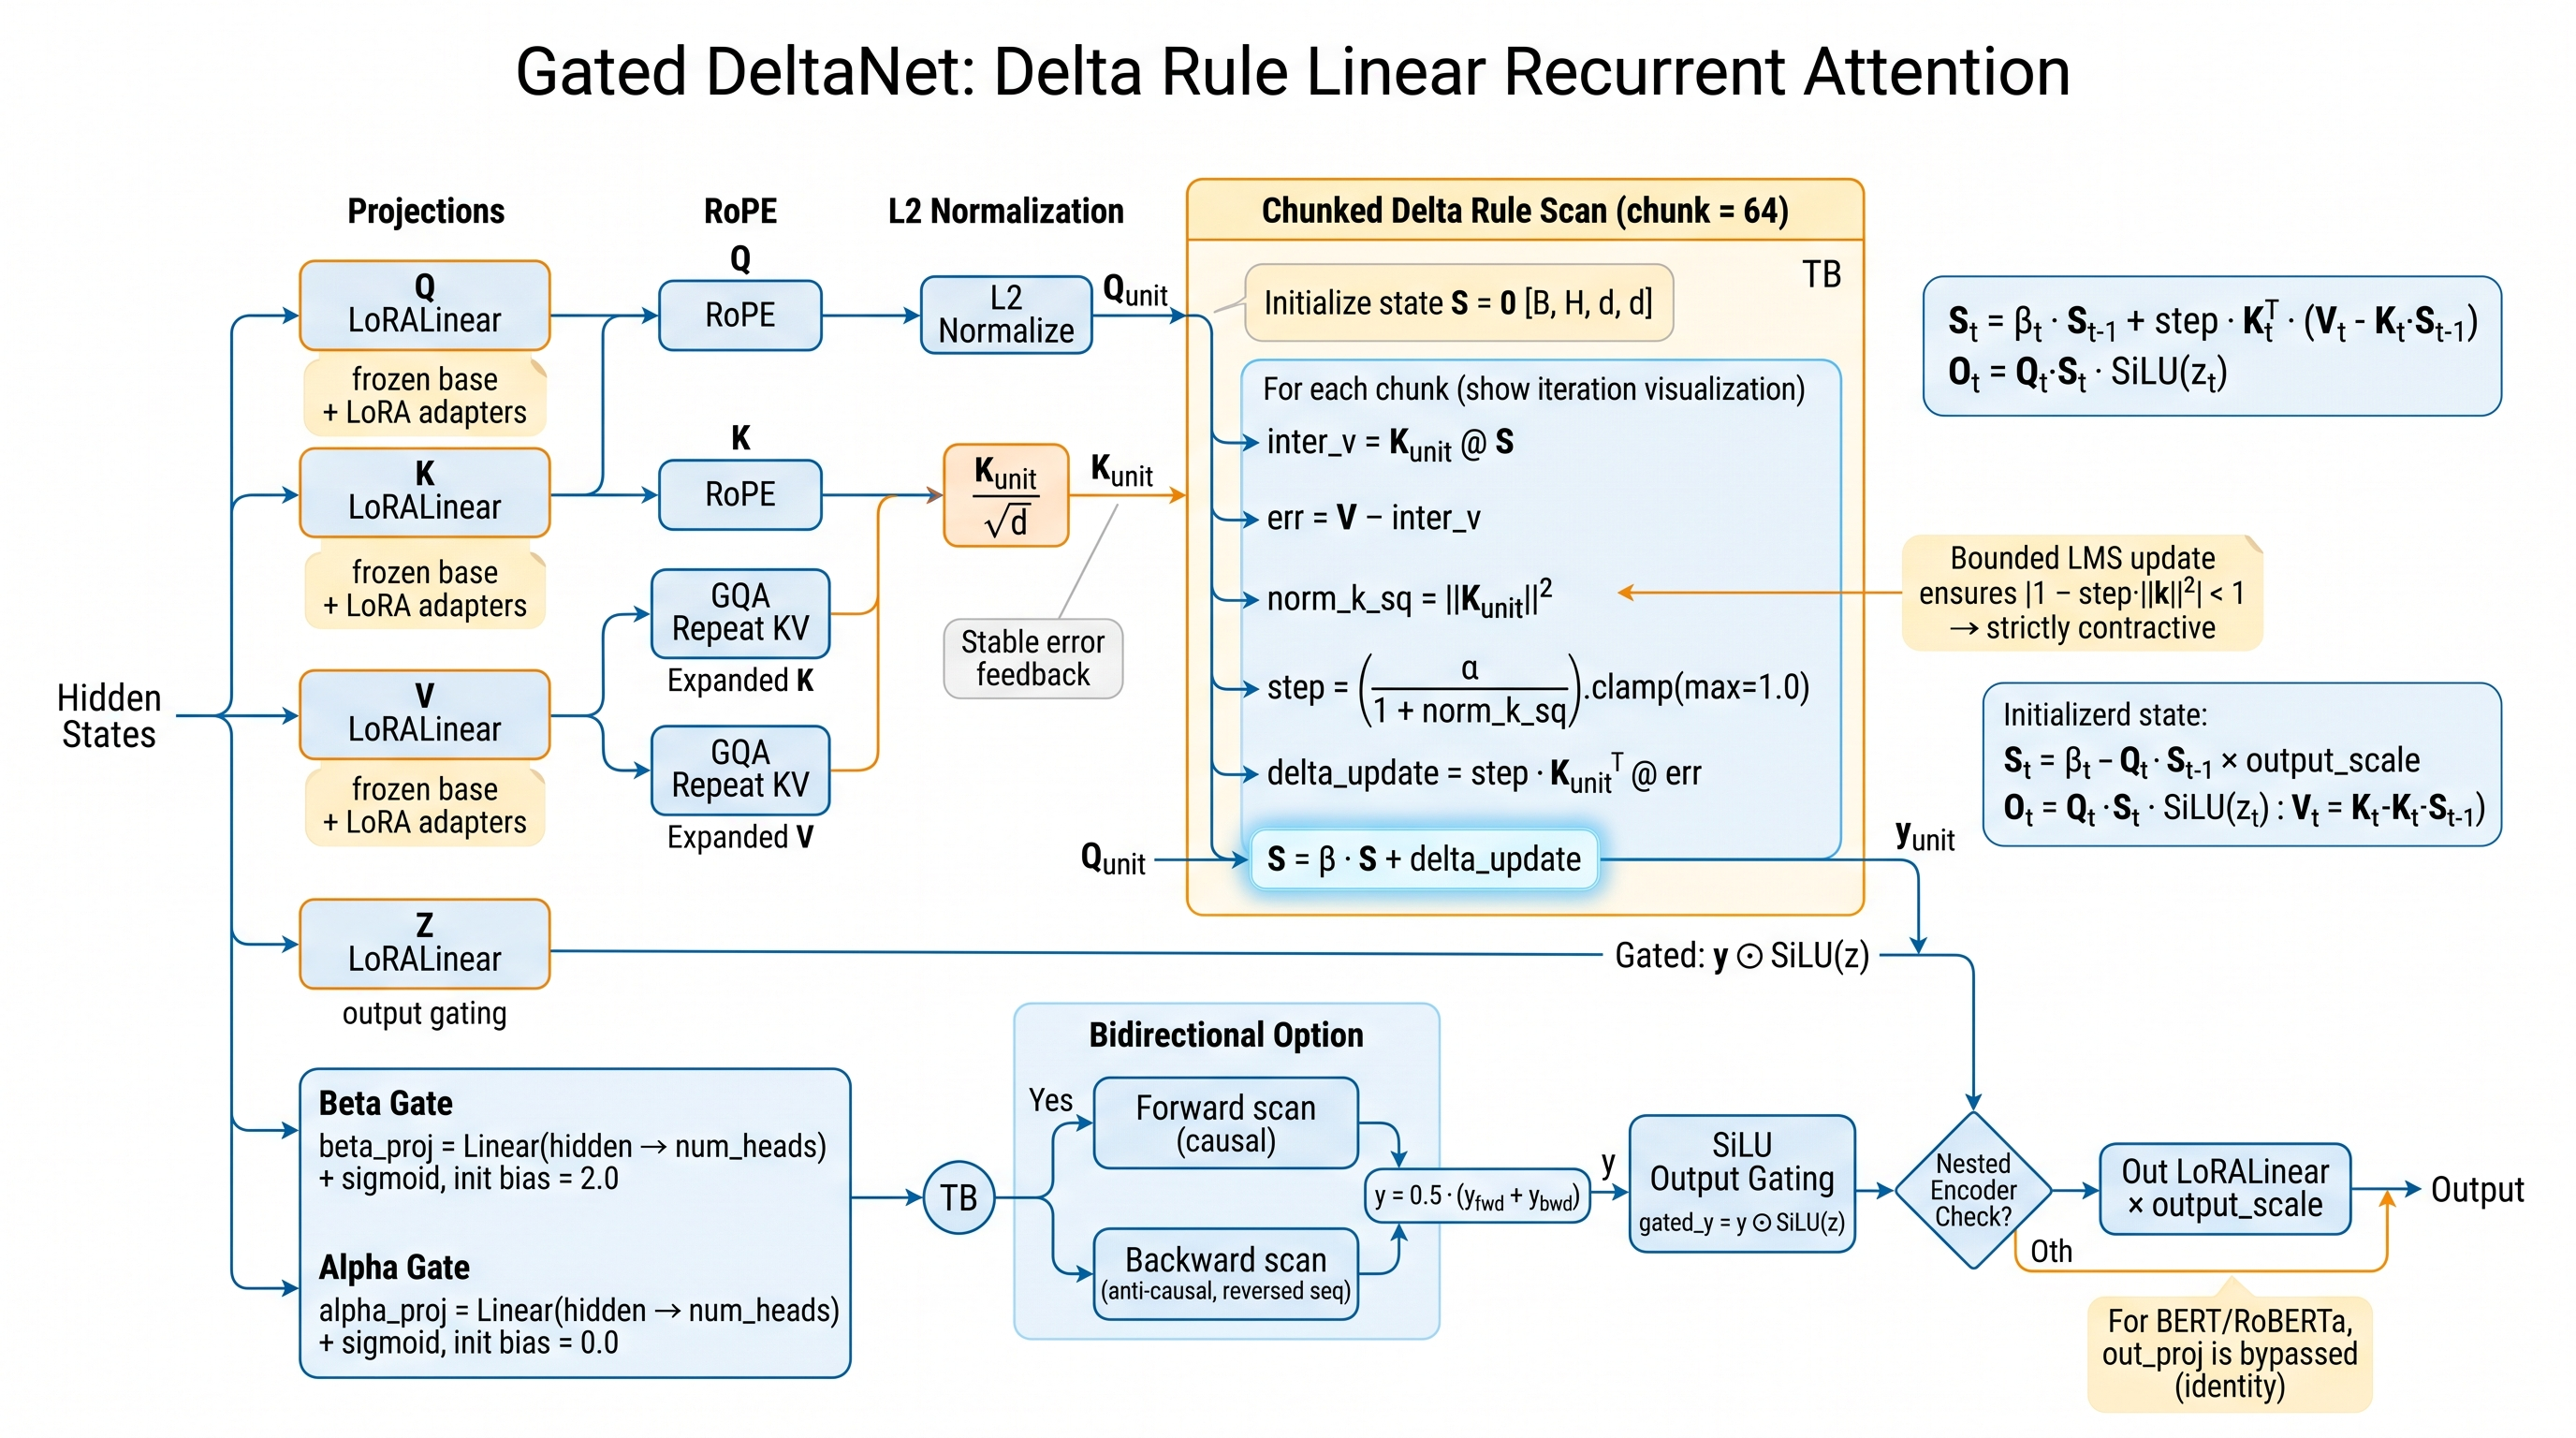
\includegraphics[width=\linewidth]{figures/architecture.jpeg}
\caption{High-level architectural diagram of gated\_delta\_net.}
\label{fig:arch_gated-delta-net}
\end{figure}

